\documentclass[12pt]{article}  % standard LaTeX, 12 point type
\usepackage{amsfonts,latexsym}
\usepackage{amsthm}
\usepackage{amssymb}
\usepackage[utf8]{inputenc} % Кодировка
\usepackage[english,russian]{babel} % Многоязычность

\newtheorem{theorem}{Theorem}[section]
\newtheorem{proposition}[theorem]{Proposition}
\newtheorem{lemma}[theorem]{Lemma}
\newtheorem{corollary}[theorem]{Corollary}
\newtheorem{conjecture}[theorem]{Conjecture}

\theoremstyle{definition}
\newtheorem{definition}{Определение}[section]
\newtheorem{example}{Example}[section]

% unnumbered environments:

\theoremstyle{remark}
\newtheorem*{remark}{Remark}
\newtheorem*{notation}{Notation}
\newtheorem*{note}{Note}

\setlength{\parskip}{5pt plus 2pt minus 1pt}
%\setlength{\parindent}{0pt}

\usepackage{color}
\usepackage{listings}
\usepackage{caption}
\usepackage{graphicx}
\usepackage{ucs}

\graphicspath{{pics/}}


\lstnewenvironment{algorithm}[1][]
{   
    \lstset{ 
        frame=tB,
        numbers=left, 
        mathescape=true,
        numberstyle=\small,
        basicstyle=\small, 
        inputencoding=utf8, 
        extendedchars=\true,
        keywordstyle=\color{black}\bfseries,
        keywords={,function, procedure, return, datatype, function, in, if, else, for, foreach, while, denote, do, and, then, assert,} 
        numbers=left,
        xleftmargin=.04\textwidth,
        #1 % this is to add specific settings to an usage of this environment (for instnce, the caption and referable label)
    }
}
{}

\newcommand{\tab}[1][0.3cm]{\ensuremath{\hspace*{#1}}}





\title{Modification of modificated CYK}
\author{Anya Yaveyn}
\date{\today}

\begin{document}


В работе~\cite{okhotin13} предложен алгоритм синтаксического анализа, основанный на перемножении матриц. 
Для того, чтобы описать модификацию этого алгоритма, в разделе~\ref{se:term} мы введем немного измененную терминологию, дальше, в разделе~\ref{se:okhotin} переформулируем оригинальный алгоритм в рамках этой терминологии. Обещанную модификацию алгоритма опишем в секции \ref{se:modification}.


\section{Терминология}
\label{se:term}
% todo: нормальное название секции

Введем обозначения, немного отличающиеся от используемых в статье~\cite{okhotin13}.
Пусть $G=(\Sigma, N, R, S)$ --- грамматика в нормальной форме Хомского и $w = a_1 \dots a_{n}$ --- строка, причем $n + 1 = 2^k$. Ограничение на длину строки (для обоих рассмотренных алгоритмов) введены скорее из соображений простоты изложения, так как оба алгоритма довольно легко обобщаются на строки произвольной длины. Далее, пусть $T$ --- треугольная матрица $n \times n$ с элементами $T[i,j] \subseteq N;\ 1 \leqslant i, j \leqslant n$. Цель алгоритма --- заполнить ячейки матрицы $T$ так, чтобы выполнялось следующее условие:
$$
T[i,j] = \{A\,|\,a_{n+1-j} \dots a_{i} \in L(A)\}, \tab \mbox{при } 1 \leqslant i, j \leqslant n < i+j\,.
$$
Вспомогательная матрица $P$ с элементами $P[i,j] \subseteq N \times N$ в результате должна быть заполнена значениями 
$$
P[i,j] = \{(B,C)\, |\, a_{n+1-j} \dots a_{i} \in L(B)L(C)\}, \tab 1 \leqslant i, j \leqslant n < i+j\,.
$$

\begin{definition}
Будем называть $(i, j)$ \textit{корректной} парой индексов, если для них выполнены условия $1 \leqslant i, j \leqslant n < i+j$.
\end{definition}

Заметим, что алгоритм в принципе рассматривает только те ячейка матриц $T$ и $P$, которые задаются корректными парами индексов.

\begin{definition}
\label{def:def_1}
Назовем \textit{(квадратной) подматрицей} такой набор корректных пар индексов $S=\{(i,j)\}$, что существуют корректная пара индексов $(a, b)$ и $size > 0$, для которых выполнены следующие условия: $size \leqslant n+1-a$, $size \leqslant n+1-b$, а также любая пара $(i,j)$, удовлетворяющая условиям $a \leqslant i < a + size$ и $b \leqslant j < b + size$, принадлежит множеству $S$. Тогда $size$ --- \textit{размер}, а пара индексов $(a,b)$ --- \textit{вершина} этой подматрицы.
\end{definition}

\begin{definition}
\label{def:def_2}
Для подматрицы $m$ с вершиной $(a,b)$ и размером $s$ определим множество индексов $\mathcal{I}_m$, \textit{влияющее на подматрицу $m$}, как 
$$\mathcal{I}_m = \{(i, j)\,|\,i < n + 1 - b,\,j < b + s\} \cup \{(i, j)\,|\,i < a + s,\,j < n + 1 - a\}\,.$$
\end{definition}


\begin{figure}[!h]
  \centering
    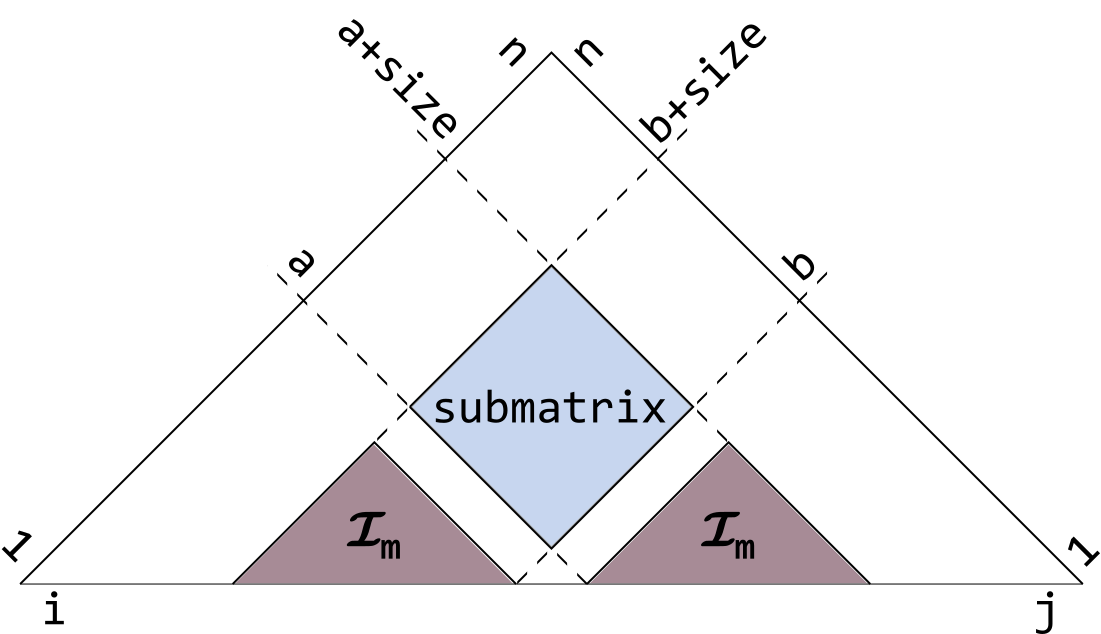
\includegraphics[width=0.9\linewidth]{submatrix.png}
  \caption{Иллюстрация к определениям~\ref{def:def_1} и \ref{def:def_2}: $(a,b)$ --- вершина подматрицы submatrix размером (size$\times$size); $\mathcal{I}_m$ --- зона, влияющая на подматрицу submatrix}
  \label{gr:submatrix}
\end{figure}

\begin{definition}
Пусть $S$ --- подматрица. Будем обозначать через $T[S]$ и $P[S]$ подматрицы матриц $T$ и $P$, соответствующие множеству индексов $S$.
\end{definition}

\pagebreak

Для описания алгоритмов нам необходимо задать ряд вспомогательных функций для оперирования подматрицами. Эти функции представлены в листинге~\ref{helpers}.

\begin{algorithm}[caption={Вспомогательные функции обработки подматриц}, label={helpers}]
function $size(m)$
function $bottomCell(m)$

function $leftSubmatrix(m)$
function $topSubmatrix(m)$
function $rightSubmatrix(m)$
function $bottomSubmatrix(m)$

function $rightNeighbor(m)$
function $leftNeighbor(m)$
function $rightGrounded(m)$
function $leftGrounded(m)$     
\end{algorithm}

Функции $size(m)$ и $bottomCell(m)$ вычисляют размер и вершину подматрицы $m$ соответственно. Следующие четыре функции $leftSubmatrix(m)$~--- $bottomSubmatrix(m)$ возвращают одну из подматриц, делящих исходную подматрицу $m$ на четыре части, как показано на рисунке \ref{gr:inner}.


\begin{figure}[!ht]
  \centering
    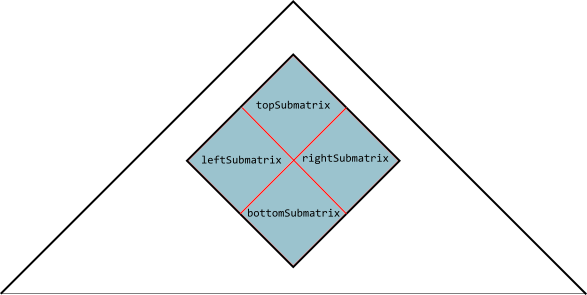
\includegraphics[width=0.9\linewidth]{inner.png}
  \caption{Иллюстрация к листингу~\ref{helpers}: разбиение матрицы на 4 компоненты}
  \label{gr:inner}
\end{figure}

\pagebreak

В свою очередь функции $rightNeighbor(m)$ и $leftNeighbor(m)$ возвращают подматрицы, сдвинутые относительно исходной на $size(m)$ по одной из осей, как показано на рисунке \ref{gr:outer}.
Функции $rightGrounded(m)$ и $leftGrounded(m)$ (рисунок \ref{gr:outer}) также возвращают подматрицы, сдвинутые относительно $m$, но на этот раз величина сдвига вычисляется по формуле $a + b - (n + 1)$, где $(a,b)$ --- вершина матрицы $m$.
Заметим, что для вершины $(i,j)$ любой их двух матриц $rightGrounded(m)$ и $leftGrounded(m)$ выполняется равенство $i + j = n + 1$. Это означает, что вершина расположена в самой <<нижней>> из использующихся диагоналей всей матрицы. 

\begin{figure}[!ht]
  \centering
    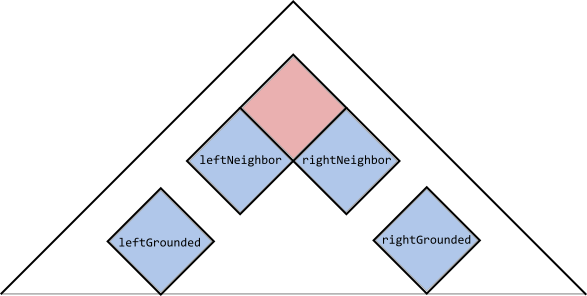
\includegraphics[width=0.9\linewidth]{outer.png}
  \caption{Иллюстрация к листингу~\ref{helpers}: соседи матрицы}
  \label{gr:outer}
\end{figure} 




\section{Алгоритм синтаксического анализа, основанный на перемножении матриц}
\label{se:okhotin}

Описание алгоритма, взятого из статьи ~\cite{okhotin13}, представлено в виде псевдокода, приведённого в следующем листинге~\ref{alg:okhotin}. 

Здесь, процедура $compute(i, j)$ принимает на вход такие $i, j$, что $(i-1,j-1)$~--- корректная пара индексов и записывает значения во все ячейки $(i', j')$ матрицы $T$ такие, что  $i' + j' > n$, $i' < i$ и $j' < j$. 

Процедура $complete(m)$, в свою очередь, принимает на вход подматрицу $m$ и определена только для подматриц с размером, являющимся степенью двойки. $complete(m)$ вычисляет все значения матрицы $T$ на переданном ей множестве индексов $m$, при выполнении некоторых дополнительных условий. Во-первых, матрица $T$ должны быть корректно заполнена для всех пар индексов из множества $\mathcal{I}_m$. Во-вторых для всех $(i,j) \in m$ текущее значение $P[i,j]$ должно быть следующим:
$$\{(B,C)\,|\,\exists k: n + 1 - b \leqslant k < a,\ a_{n+1-j}\dots a_k \in L(B) \mbox{ и } a_{k+1}\dots a_i \in L(C)\}\,,$$
где $(a,b)$~--- вершина подматрицы $m$.

\begin{algorithm}[caption={Алгоритм синтаксического анализа, основанный на перемножении матриц}, label={alg:okhotin}] 
procedure $main()$:
    $compute(n + 1, n + 1)$
    
procedure $compute(i, j)$:
    if $i + j - n \geqslant 4$ then
        $compute\left(i, \frac{j}{2}\right)$
        $compute\left(\frac{i}{2}, j\right)$
    denote $m = submatrixByBottomCellAndSize\left(\left(\frac{n + i - j}{2},\frac{n + j - i}{2}\right),\ \frac{i + j - n}{2}\right)$
    $complete(m)$
    
procedure $complete(m)$
    denote $(i, j) = bottomCell(m)$
    if $size(m) = 1$ and $i + j = n$ then
        $T[i,j] = \{A\,|\,A\to a_i \in R\}$
    else if $size(m) = 1$ then
        $T[i,j] = f(P[i,j])$
    else if $size(m) > 1$ then
        denote $\mathcal{B} = bottomSubmatrix(m)$, $\mathcal{L} = leftSubmatrix(m)$,
               $\mathcal{R} = rightSubmatrix(m)$, $\mathcal{T} = topSubmatrix(m)$
        $complete(\mathcal{B})$
        $P[\mathcal{L}] = P[\mathcal{L}] \cup \left(T[leftGrounded(\mathcal{L})] \times T[\mathcal{B}]\right)$
        $complete(\mathcal{L})$
        $P[\mathcal{R}] = P[\mathcal{R}] \cup \left(T[\mathcal{B}] \times T[rightGrounded(\mathcal{R})]\right)$
        $complete(\mathcal{R})$
        $P[\mathcal{T}] = P[\mathcal{T}] \cup \left(T[leftGrounded(\mathcal{T})] \times T[\mathcal{R}]\right)$
        $P[\mathcal{T}] = P[\mathcal{T}] \cup \left(T[\mathcal{L}] \times T[rightGrounded(\mathcal{T})]\right)$
        $complete(\mathcal{T})$
\end{algorithm}

\section{Модифицированный алгоритм}
\label{se:modification}

Далее предложена модификация исходного алгоритма синтаксического анализа, предназначенная для его более естественной адаптации к задаче поиска подстрок, выводимых в заданной грамматике.

Главная процедура $main$ сначала обрабатывает нижний слой матрицы $T$ (клетки $(i,j)$, для которых $i+j=n+1$), записывая в него корректные значения. Потом разбивает матрицу $T$ на слои, как показано на картинке \ref{gr:layers} (каждый слой состоит из набора подматриц, у каждой из которых отброшена нижняя четверть --- $bottomSubmatrix$). Полученные слои обрабатываются последовательно снизу вверх, с помощью процедуры $completeVLayer$, заполняя тем самым всю матрицу $T$.

\begin{figure}[!ht]
  \centering
    
\includegraphics[width=0.9\linewidth]{layers.png}
  \caption{Первичное разбиение на слои}
  \label{gr:layers}
\end{figure}


Процедура $completeVLayer$, в свою очередь, принимает на вход набор подматриц $M$. Эти подматрицы не должны пересекаться, а также для любых двух подматриц $m_1, m_2 \in M$; $(a_i,b_i),\ s_i$~--- вершина и размер $m_i$ соответственно, должно выполняться $s_1 = s_2$ и $a_1 + b_1 = a_2 + b_2$. Для каждого элемента $m$ множества $M$ процедура достраивает матрицу $T$ для трех верхних четвертей ($leftSubmatrix(m)$, $rightSubmatrix(m)$ и $topSubmatrix(m)$). Для корректной работы этой функции, во-первых, необходимо, чтобы для любой $m \in M$ ячейки $T[i,j]$ были построены  для $(i,j) \in\ bottomSubmatrix(m)$ и для $(i,j) \in\ \mathcal{I}_m$. Во-вторых, требуется удовлетворение ограничения на матрицу $P$, аналогичного ограничению в случае процедуры $complete$ оригинального алгоритма, а именно: для любой $m \in M$ и для всех $(i,j) \in m$ текущее значение $P[i,j]$ должно быть следующим:
$$\{(B,C)\,|\,\exists k: n + 1 - b \leqslant k < a,\ a_{n+1-j}\dots a_k \in L(B) \mbox{ и } a_{k+1}\dots a_i \in L(C)\}\,,$$
где $(a,b)$~--- вершина подматрицы $m$.

Третья процедура --- $completeLayer$ --- тоже принимает на вход набор подматриц $M$, но для каждого элемента $m$ этого набора достраивает матрицу $T$ для всей подматрицы $m$. Ограничения на входные данные такие же, как и у процедуры $completeVLayer$. Для корректной работы этой функции необходимо, чтобы для любой $m \in M$ ячейки $T[i,j]$ были построены для $\mathcal{I}_m$, а так же выполнение того же требования на $P$, что и в предыдущем случае. 

\begin{algorithm}[caption={Алгоритм}, label={main}]
procedure $main()$:
  for $\ell$ in $(1,\,\dots,\,n)$ do
    $T[\ell, n+1-\ell] = \{A\,|\,A \to a_{\ell} \in R\}$
  foreach $1 \leqslant i < k$ do
    denote layer = $constructLayer(i)$
    $completeVLayer($layer$)$  

procedure $completeLayer(M)$:
  if $\forall\ m \in M$, $size(m) = 1$ then
    denote cells = $\{bottomCell(m)\,|\, m \in M\}$
    foreach $(x, y) \in $ cells do
      $T[x, y] = f(P[x, y])$
  else
    denote bottomLayer = $\{bottomSubmatrix(m)\,|\,m \in M\}$
    $completeLayer($bottomLayer$)$
    $completeVLayer(M)$     

procedure $completeVLayer(M)$:
  denote leftSubLayer = $\{leftSubmatrix(m)\,|\,m \in M\}$
  denote rightSubLayer = $\{rightSubmatrix(m)\,|\,m \in M\}$
  denote topSubLayer = $\{topSubmatrix(m)\,|\,m \in M\}$

  foreach $m \in$ leftSubLayer do
    $P[m] = P[m] \cup (T[leftGrounded(m)] \times T[rightNeighbor(m)])$
  foreach $m \in$ rightSubLayer do
    $P[m] = P[m] \cup (T[leftNeighbor(m)] \times T[rightGrounded(m)])$

  $completeLayer($leftSubLayer $\cup$ rightSubLayer$)$

  foreach $m \in$ topSubLayer do
    $P[m] = P[m] \cup (T[leftGrounded(m)] \times T[rightNeighbor(m)])$
  foreach $m \in$ topSubLayer do
    $P[m] = P[m] \cup (T[leftNeighbor(m)] \times T[rightGrounded(m)])$

  $completeLayer($topSubLayer$)$  
\end{algorithm}

Процедура $main$ реализуется через $completeVLayer$ очевидным образом. Для построения множества подматриц, составляющий слой под номером $i$ используется функция $constructLayer(i)$, реализация которой оставлена за скобками. Процедура $completeLayer$ по сути аналогична процедуре $complete$ из статьи, за исключением того, что она выполняется сразу для нескольких матриц. Таким же образом отдельно разбирается случай, когда переданные матрицы имеют размер $1 \times 1$. Иначе матрицы разбиваются на четыре части и сначала следует рекурсивный вызов от $bottomSubmatrix$ (для всех переданных матриц), а затем вызов процедуры $completeVLayer$, которая обрабатывает верхние части матриц. 

Процедура $completeVLayer$ для каждой из переданных матриц сначала выполняет два перемножения (соответствует 21 и 23 строкам в алгоритме из статьи), затем вызывает $completeLayer$ от $rightSubmatrix$ и $leftSubmatrix$ (22 и 24 строки оригинального алгоритма), далее выполняет оставшиеся два умножения (строки 25 и 26) и, наконец, вызывает $completeLayer$ от оставшейся части $topSubmatrix$ (строка 27).

% Наверное надо сказать пару слов о том. почему эти алгоритмы делают одно и то же?...

\section{Заключение}

Заметим, что если мы хотим адаптировать алгоритм для задачи поиска подстроки длины не большей, чем какое-то заданное $m \ll n$, тогда нам надо строить матрицы $T$ и $P$ только для индексов $i + j \leqslant n + m$. В этом случае в оригинальном алгоритме придется производить большое количество <<холостых>> рекурсивных вызовов. В модифицированном алгоритме этого отчасти можно избежать, изменив верхнюю границу в цикле for (строка 4 листинга \ref{main}).

Также представленная модификация алгоритма собирает вместе все умножения матриц одного размера (и расположенных на одном <<уровне>>), которые можно сделать независимо друг от друга. Это позволяет более эффективно распараллеливать эти умножения.

\begin{thebibliography}{9}

\bibitem{okhotin13}
  Alexander Okhotin,
  ``Parsing by matrix multiplication generalized to Boolean grammars'',
  \emph{Theoretical Computer Science},
  V. 516,
  p. 101--120,
  January 2014

\end{thebibliography}

\end{document}